\documentclass[11pt]{article}

\usepackage{booktabs}
\usepackage{homeworkpkg}
\usepackage{enumitem}
\usepackage{xcolor,listings}
\usepackage{caption}
\usepackage{multirow}
\usepackage{amsmath}
\usepackage{multicol}

\graphicspath{ {images/} }

%% Local Macros and packages: add any of your own definitions here.

\begin{document}

% Homework number, your name and NetID, and optionally, the names/NetIDs of anyone you collaborated with. If you did not collaborate with anybody, leave the last parameter empty.
\homework
    {5}
    {Nestor Alejandro Bermudez Sarmiento (nab6)}
    {}


\section*{Introduction}

In this assignment we explore two topics: classifications methods and clustering methods.
For classification we will illustrate the use of a Naive Bayes classifier and also K-nearest neighbor using different values of $k$. Finally we will look at the k-means, DBSCAN and AGNES clustering algorithms.

\section*{Question 1}

Consider the following equations:\\
\begin{gather}
Pr(X, C) = Pr(X \mid C) \times Pr(C) \\	
Pr(C \mid X) = \frac{Pr(X \mid C) \times Pr(C)}{Pr(X)}
\end{gather}

\textbf{1a(i)}: $Pr$(Popularity = `P') = $\frac{7}{10}$. Done by simply counting the number of examples that match the criteria. Known as the prior probability.\\

\textbf{1a(ii)}: $Pr$(Popularity = `NP') = $\frac{3}{10}$. Found by taking the value from the previous question from 1 since this is a binary classification problem.\\

\textbf{1a(iii)}: By using equation 1 and class-conditional independence:
\[ Pr(\textrm{Price = `\$', Delivery = `Yes' , Cuisine = `Korean' \textbar{} Popularity = `P'}) \]
\[ = \prod_{i=1}^3 Pr(x_i \mid \textrm{Popularity = `P'}) \]
where $x_i$ is each of the features in the tuple considered. So:\\
\[ x_1 = \frac{4}{7}, x_2 = \frac{4}{7}, x_3 = \frac{2}{7} \] and then
\[ Pr(\textrm{Price = `\$', Delivery = `Yes' , Cuisine = `Korean' \textbar{} Popularity = `P'}) = \frac{4}{7} \times \frac{4}{7} \times \frac{2}{7} = \frac{32}{343} \]

\textbf{1a(iv)}: $Pr$(Price = `\$', Delivery = `Yes' , Cuisine = `Korean' \textbar{} Popularity = `NP')
\[ = \prod_{i=1}^3 Pr(x_i \mid \textrm{Popularity = `P'}) \]
where $x_i$ is each of the features in the tuple considered. So:\\
\[ x_1 = \frac{1}{3}, x_2 = \frac{2}{3}, x_3 = \frac{1}{3} \] and then
\[ Pr(\textrm{Price = `\$', Delivery = `Yes' , Cuisine = `Korean' \textbar{} Popularity = `P'}) = \frac{4}{7} \times \frac{4}{7} \times \frac{2}{7} = \frac{2}{27} \]

\textbf{1b}: When doing Naive Bayes classification one of the common ways to perform the prediction is to using \textbf{MAP}\footnote{\url{https://en.wikipedia.org/wiki/Maximum_a_posteriori_estimation}} (Maximum a posteriori). MAP indicates that we should calculate the probability of each class given the evidence. For this particular case, we have already done that in part 1a(iii) and 1a(iv). \\

So to answer the question it is just enough to compare the previous results. Since $\frac{32}{343} > \frac{2}{27}$ the answer to the question is \textbf{yes}, it will be class as Popular.\\

\textbf{1c}: the techniques we discussed in class can, theoretically, apply to Naive Bayes. That is: boosting, bagging and ensemble. There is no "one size fit all" solution and finding the right method usually involves trying multiple of them until you get a reasonable accuracy. One of the algorithms we can use is AdaBoost on top of Naive Bayes. This works as follows: \\

Let $d$ be the number of classes and $k$ the number of iterations or predictors in our ensemble method. These will be the hyper-parameters of our classifier.
\begin{enumerate}
\item make all tuples equally likely, e.g. assign the same weight to all of them. The usual value for the weigh is the inverse of the number of classes ($\frac{1}{d}$).
\item create a new data set $D_i$ by sampling with replacement from the original data set. Whether an example is included or not in $D_i$ is decided by its weigh. 
\item train a Naive Bayes classifier using $D_i$.
\item evaluate the Naive Bayes classifier and find its error rate. We can do it by using the test data or by using some of the examples that were not included in $D_i$. 
\item if the error is greater than a threshold (at least 50\%), reset the weighs and try again with a new sample (go back to step 2).
\item if the error is good enough then for every tuple in $D_i$ update its corresponding weigh by a factor of the $\frac{e}{acc}$ where $e$ is the error and $acc$ is the accuracy ($1 - e$).
\item repeat from step 2 if done less than $k$ times.
\end{enumerate}

Once the training is done we need to predict labels for new evidence \textbf{X}. To do so we initialize the weights with zero and on each iteration we update them by taking the log of the accuracy over the error rate. On each iteration we see what the prediction for the current classifier is and update the weight of that class only! At the end we predict the class with the highest weight.\\

\textbf{1d}: There are a few metrics that can help measure the performance of a classifier when one of the classes is rare.\\

i) Sensitivity: it measures the rate of true positives recognition and is defined by the formula: $\frac{TP}{P}$. Where TP is the total number of true positives (correctly classified as positive) and P is the total number of instances that were positive. Note that the formula does not include the negatives so it ignores the fact that the positives are rare because there is no point of comparison between positives and negatives.\\

ii) Specificity: measures how successful is the classifier in predicting false when over the examples that were indeed false. As an example, in a medical diagnosis, tests usually have high specificity, meaning that they rarely predict a positive in healthy patients, this doesn't say much about whether it was positive or not but it is a first step to perform more tests. Example inspired by this Wikipedia \href{https://en.wikipedia.org/wiki/Sensitivity_and_specificity#Sensitivity}{page}

\section*{Question 2}

\textbf{2a}: since $k = 1$ this is rather simple. For every example in the test data we calculate the distance to every exampled seen in the training data. The following table summarizes this and marks the minimum distance in green.
\begin{center}
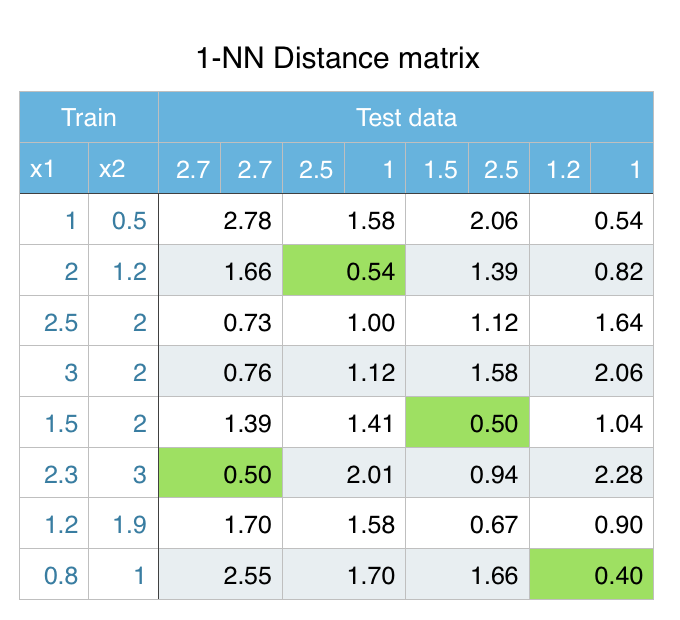
\includegraphics[scale=0.75]{distances.png}
\end{center}

The first 4 rows in the matrix correspond to the training examples that belong to class +1 and the other half the ones that belong to class -1. So, the predicted classes for the test data are: -1, +1, -1 and -1 respectively. And the actual classes are +1, +1, -1, -1 so only the first one was miss-classified and, therefore, the accuracy is $\frac{3}{4} = $ \textbf{0.75} and the error is \textbf{25\%}.\\

\textbf{2b}: when using $k = 3$ the distance matrix doesn't change but now 3 points "vote" to decide the class to assign to each example. The 3 closest points to each test example are highlighted in green in the following table:
\begin{center}
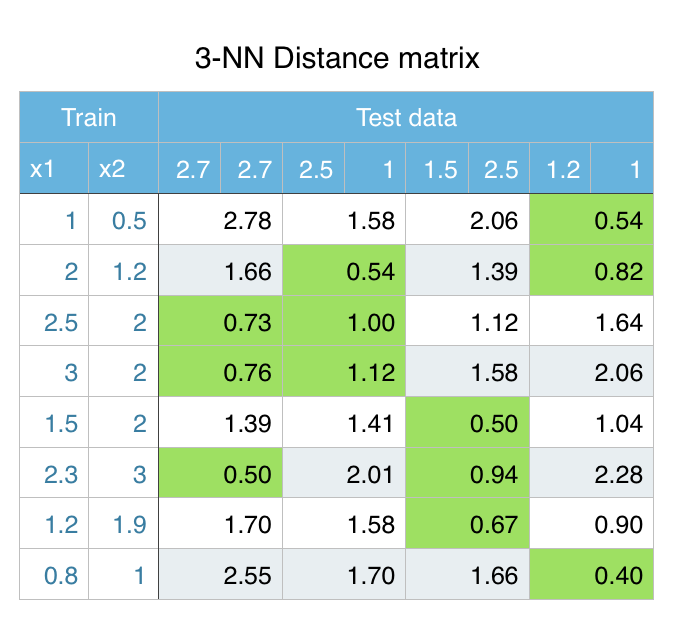
\includegraphics[scale=0.75]{3-nn-distances.png}
\end{center}
So for the first test example (2.7, 2.7) two of the three closest points are +1 so it will be classified as +1; for the second example (2.5, 1) all three points are +1 so its class is +1; for (1.5, 2.5) all three are -1 so its class -1 and, finally, (1.2, 1) will be classified as +1. \\
Only the last prediction is wrong so the accuracy of the model in this case is also \textbf{0.75} and the error rate is \textbf{25\%}.\\

\textbf{2c}: lets look at the scatter plot shown in the HW description.
\begin{center}
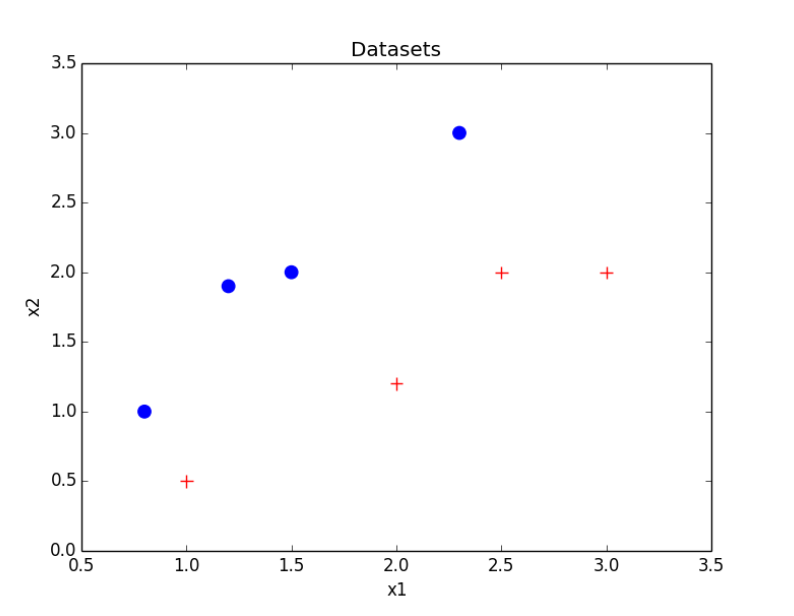
\includegraphics[scale=0.55]{q2-dataplot-ref.png}
\end{center}

What I'll do to find the linear classifier is to take the two points on the bottom-left corner, draw the line that joins them (lets call it $L_1$), take the midpoint ($M_1$) and find the perpendicular line ($L_2$) to $L_1$ that passes through $M_1$. The next image illustrates this:
\begin{center}
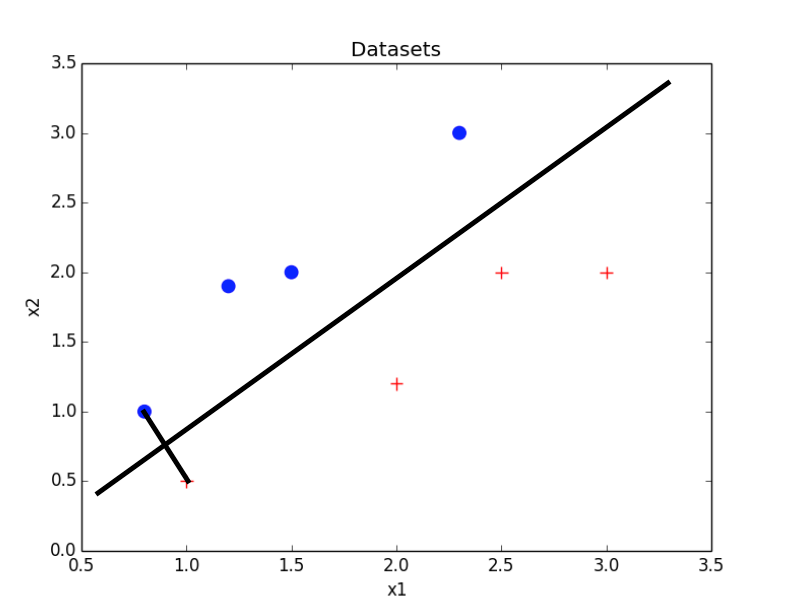
\includegraphics[scale=0.75]{q2-dataplot.png}
\end{center}

The two points into consideration are (0.8, 1) and (1, 0.5). The first one belongs to class +1. The slope of $L_1$ is given by 
\[ m_1 = \frac{x2_+ - x2_-}{x1_+ - x1_-} = \frac{1 - 0.5}{0.8 - 1} = -2.5 \]

And the midpoint $M_1$ is given by
\[ (\frac{x1_+ + x1_-}{2}, \frac{x2_+ + x2_-}{2}) = (0.9, 0.75) \]

Finally, to find a perpendicular to a line we need the product of the slopes to be -1. So the slope of $L_2$ is 0.4. So $x2 = 0.4x1 + b$, when evaluating in the midpoint we have that $0.75 = 0.4\times 0.9 + b \rightarrow b = 0.39 $. As a result the line we are looking for is:
\[ f(x) = 0.4x_1 - x_2 + 0.39 \]

The following table shows the value resulting of evaluating $f(x)$ on each data example (both training and test).

\begin{center}
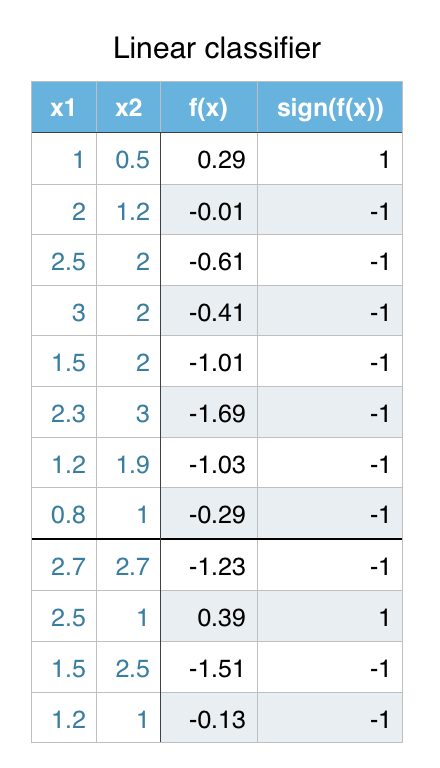
\includegraphics[scale=0.75]{linear.png}
\end{center}

I was expecting to see a perfect accuracy but it wasn't the case. After a while I realized that the problem is that the scale on the axis x1 and x2 in the scatter plot are not equal so, even though $L_2$ seemed like a good fit it really wasn't. The accuracy for the training data set is $\frac{5}{8} = 62.5\%$ while the accuracy in the test data set is \textbf{75\%}.\\

A different way to find $f(x)$ would be to take the same midpoint $M_1$ we already found and take a second midpoint from the segment that joins (1.2, 1.9) and (2, 1.2). The reason for choosing these two points is that it looks like line drawn before passes through its midpoint. Lets call this point $M_2$. Its coordinate would be (1.7, 1.95). \\

Now we just need to find a line that passes through $M_1$ and $M_2$. Following the same steps as before we have that $f(x) = 1.5x1 - x2 - 0.6$.\\

Now lets look at the table evaluating the function on all the examples.
\begin{center}
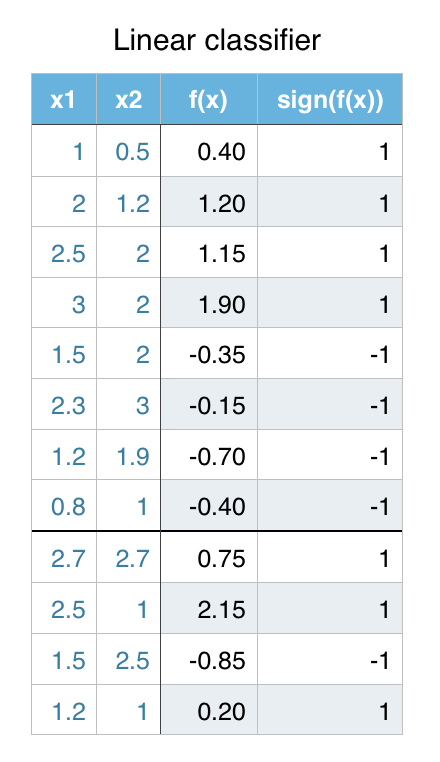
\includegraphics[scale=0.75]{linear2.png}
\end{center}

This time the accuracy on the training data set is \textbf{100\%} and the accuracy on the test data set is \textbf{75\%}. Since the question is asking about the error:\\
Training error is \textbf{0\%}\\
Testing error is \textbf{25\%}\\

\textbf{2d}: for this particular data set both method perform equally well. In general $k$ Nearest Neighbor is good when you have low dimensional data and many examples but this is not the case here; we do have low dimensional data but also just a few examples. As mentioned earlier in this report, there is no "one size fit all" solution and you usually have to experiment with different methods. Regardless of that, there are some particular scenarios in which one is better than the other. When we have lots of data entries KNN may not be a good fit because the computational complexity could explode. 

\section*{Question 3}

\end{document}
